% Chapter Template

\chapter{Introduction} % Main chapter title

\label{Chapter1} % Change X to a consecutive number; for referencing this chapter elsewhere, use \ref{ChapterX}

%----------------------------------------------------------------------------------------
%	SECTION 1
%----------------------------------------------------------------------------------------

\section{Laminated Composite Material}

Composite materials offer improved strength, stiffness, corrosion resistance,
etc. over conventional materials, and are widely used as alternative materials
for applications in various industries ranging from electronic packaging to golf
clubs, and medical equipment to homebuilding, making aircraft structure to space
vechicles. The stacking sequence and fiber orientation of composite laminates
give the designer additional 'degree of freedom' to tailor the design with
respect to strength or stiffness.  One widely known advange of using composite
material is can significantly reducing the weight of target structure, and many
researchers attempted to improve the efficiency of using composite materail by
mimimizing the thickness.

Classic lamination theory(CLT) is used to develop the stress-strain relationship of
composite material under in-plane and out-of-plane loading. First, develop
stress-strain relationships, elastic moduli, strengths of an angle ply based on
a unidirectional lamina and the angle of the ply; second, becasue a laminate is
consist of more than one lamina bonded together through their thickness, so the
macromechianical analysis will be developed for a laminate based on applied
loading.  To check whether a designed lay-up is plausible or not, different
failure theories have been developed.

\section{Introduction}
Fiber-reinforced composite materials have been widely used in many industries
because they offer improved mechanical stiffness, strength, and low specific
gravity of fibers  over conventional materials. The use of composite material
materials in structural application is range from electronic packaging, sports
equipment, homebuilding, medical prosthetic devices, to high performance
military structures. The stacking sequence, ply thickness, and fiber
orientation of composite laminates give the designer additional ’degree of
freedom’ to tailor the design with respect to strength or stiffness. Classic
lamination theory(CLT) is taken to predict the behavior of a laminate from a
knowledge of the composite laminate properties of the individual layers and the
laminate geometry.

Evolutionary artificial neural networks(EANN's) is a special class of artifical
neural networks(ANN's) in which evolutionary algorithms(ES's) are introduced to
learn the optimal ANN. EA's can be used in the ANN at three different levels:
connection weights, architectures, input features, and learning rules. It is
shown, the combinations of ANN's and EA's can significantly improve the
performance of intelligent systems that rely's on ANN's or EA's alone.



The rest of the paper is organized as follows. Section 2 explains the classical
laminate theory and the failure criteria taken in the present study. Section 3
explains the design of artifical neural network for mathmatical model
approximation.  Section 4 reviews the use of genetic algorithm in the design of
neural network architecture and the parameters optimization during the training
process of neural network.  design Section 4 describes the result of the
numerical experiments in different cases, and in the Conclusion section we
dicuss the results.
\section{Classic Lamination Theory}
Classical lamination theory is based upon three simplifying engineering
assumptions: (1) Each layer's thickness is very small and consist of
homogeneous, orthotropic material, and these layers are prefectly bonded
together; (2) The entire laminated composite is supposed to be under plane
stress; (3) Normal cross sections of the entire laminate is normal to the
deflected middle surface, and do not change in thickness.
\begin{figure}
\centering
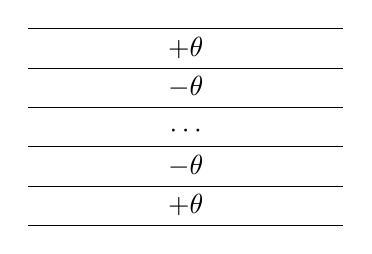
\begin{tikzpicture}
	\draw (0,0) -- (4,0);
	\draw (0,-0.5) -- (4,-0.5) node[midway, above] {$\mathit{+}\theta$};
	\draw (0,-1) -- (4,-1) node[midway, above] {$\mathit{-}\theta$} ;
	\draw (0,-1.5) -- (4,-1.5) node[midway, above] {$\cdots$};
	\draw (0,-2) -- (4,-2) node[midway, above] {$\mathit{-}\theta$};
	\draw (0,-2.5) -- (4,-2.5) node[midway, above] {$\mathit{+}\theta$};
\end{tikzpicture}
\caption{Model for Angle ply laminate}
\end{figure}

\subsection{Stress and Strain in a Lamina}
For a single lamina has a small thickness under plane stress, and it's upper and lower surfaces of the lamina are
free from external loads. According to the Hooke's Law, the three-dimensional stress-strain equations can be reduced to
two-dimensional stress-strain equations. The stress-strain relation in local axis 1-2 is:
\begin{equation}
    \begin{bmatrix}
        \sigma _1\\
        \sigma _2\\
        \tau_{12}
    \end{bmatrix}
    =
    \begin{bmatrix}
        Q_{11} & Q_{12} & 0\\
        Q_{12} & Q_{22} & 0\\
        0      &  0     & Q_{66}
    \end{bmatrix}
    \begin{bmatrix}
        \varepsilon_1\\
        \varepsilon_2\\\gamma_{12}
    \end{bmatrix}
\end{equation}
where $Q_{ij} $are the stiffnesses of the lamina that are related

to engineering elastic constants given by
\begin{equation}
    \begin{split}
    &Q_{11}=\frac{E_1}{1-v_{12}v_{21}}\\
    &Q_{22}=\frac{E_2}{1-v_{12}v_{21}}\\
    &Q_{66}=G_{12}\\
    &Q_{12}=\frac{v_{21}E_2}{1-v_{12}v_{21}}\\
    \end{split}
\end{equation}

where $E_1, E_2, v_{12}, G_{12} $ are four independent engineering elastic constants, which are defined as follows: $E_1 $ is the longitudinal Young's modulus, $E_2 $ is the transverse Young's modulus, $v_{12} $ is the major Poisson's ratio, and $G_{12} $ is the in-plane shear modulus.

Stress strain relation in the global x-y axis:
\begin{equation}
	\label{equ:stress-strain}
	\left[\begin{array}{l}
			\sigma _{x} \\ \sigma _{y} \\
			\tau_{xy}\end{array}\right]=\left[\begin{array}{lll}\bar{Q}_{11} &
			\bar{Q}_{12} & \bar{Q}_{16}\\ 
			\bar{Q}_{12} & \bar{Q}_{22} & \bar{Q}_{26} \\
								\bar{Q}_{16} & \bar{Q}_{26}
			 &\bar{Q}_{66}\end{array}\right]\left[\begin{array}{l}\varepsilon_{x}
	 \\ \varepsilon_{y}\\ \gamma_{x y}\end{array}\right] \end{equation}
where
\begin{equation}
	\begin{array}{l}
		\resizebox{.35\textwidth}{!}{$\bar{Q}_{11}=Q_{11} cos^{4}\theta+Q_{22} sin^{4}\theta+2\left(Q_{12}+2
		Q_{66}\right) sin^{2}\theta cos^{2}\theta$} \\

		\resizebox{.35\textwidth}{!}{$\bar{Q}_{12}=\left(Q_{11}+Q_{22}-4 Q_{66}\right) sin^{2}\theta
		cos^{2}\theta+Q_{12}\left(cos^{4}\theta+sin^{2}\theta \right)$} \\

		\resizebox{.35\textwidth}{!}{$\bar{Q}_{22}=Q_{11} sin^{4}\theta+Q_{22} cos^{4}\theta+2\left(Q_{12}+2
		Q_{66}\right) sin^{2}\theta cos^{2}\theta$} \\

		\resizebox{.4\textwidth}{!}{$\bar{Q}_{16}=\left(Q_{11}-Q_{12}-2
		Q_{66}\right) cos^{3}\theta sin\theta-\left(Q_{22}-Q_{12}-2Q_{66}\right)
	sin^{3}\theta cos\theta$} \\ 
		\resizebox{.4\textwidth}{!}{$\bar{Q}_{26}=\left(Q_{11}-Q_{12}-2
		Q_{66}\right) cos\theta sin^{3}\theta-\left(Q_{22}-Q_{12}-2
Q_{66}\right)cos^{3}\theta sin\theta$}
		 \\ 
	\resizebox{.4\textwidth}{!}	{$\bar{Q}_{66}=\left(Q_{11}+Q_{22}-2 Q_{12}-2 Q_{66}\right)
	sin\theta^{2}cos\theta^{2}+Q_{66}\left(sin\theta^{4}+cos\theta^{4}\right)$}\\
	\end{array}
\end{equation}



The local and global stresses in an angle lamina are related

to each other through the angle of the lamina $\theta $
\begin{equation}\left[\begin{array}{l}\sigma _{1} \\ \sigma _{2} \\ \tau_{12}\end{array}\right]=[T]\left[\begin{array}{l}\sigma _{x} \\ \sigma _{y} \\\tau_{xy}\end{array}\right]
\end{equation}

where
\begin{equation}
	[T]=\left[\begin{array}{ccc}cos^{2}\theta & sin^{2}\theta & 2
		sin\theta cos\theta \\ 
sin^{2}\theta & cos^{2}\theta & -2 sin\theta cos\theta \\
-sin\theta cos\theta
			  & sin\theta cos\theta  &cos^{2}\theta -sin^{2}\theta
\end{array}\right] 
\end{equation}



\subsection{Stress and Strain in a Laminate}
For forces and moment resultants acting on laminates, such as in plate and shell
structures, the relationship between applied forces and moment and displacement
can be given by

\begin{equation} \label{eq:force_and_moments}
	\begin{array}{l}
		\begin{aligned}
	\begin{bmatrix}
		N_x \\
		N_y \\
		N_{xy}
	\end{bmatrix}
	&=
	\begin{bmatrix}
		A_{11} & A_{12} & A_{16} \\
		A_{12} & A_{22} & A_{26} \\
		A_{16} & A_{26} & A_{66} 
	\end{bmatrix}
    \begin{bmatrix}
		\varepsilon_x^0 \\
        \varepsilon_y^0 \\
		\gamma_{xy}^0
    \end{bmatrix}   \\
	&+               
	\begin{bmatrix}
		B_{11} & B_{12} & B_{16} \\
		B_{11} & B_{12} & B_{16} \\
		B_{16} & B_{26} & B_{66} 
	\end{bmatrix}
	\begin{bmatrix}
		k_x \\
		k_y \\
		k_{xy} 
	\end{bmatrix}  \\
\end{aligned} \\ \\
\begin{aligned}
	\begin{bmatrix}
		M_x \\
		M_y \\
		M_{xy}
	\end{bmatrix}
	&=
	\begin{bmatrix}
		B_{11} & B_{12} & B_{16} \\
		B_{12} & B_{22} & B_{26} \\
		B_{16} & B_{26} & B_{66} 
	\end{bmatrix}
    \begin{bmatrix}
		\varepsilon_x^0 \\
        \varepsilon_y^0 \\
		\gamma_{xy}^0
    \end{bmatrix} \\ 
	&+  
	\begin{bmatrix}
		D_{11} & D_{12} & D_{16} \\
		D_{11} & D_{12} & D_{16} \\
		D_{16} & D_{26} & D_{66} 
	\end{bmatrix}
	\begin{bmatrix}
		k_x \\
		k_y \\
		k_{xy} 
	\end{bmatrix}
\end{aligned}
	\end{array}
\end{equation}


$N_x,N_y $  - normal force per unit length

$N_{xy} $  - shear force per unit length

$M_x, M_y $ - bending moment per unit length

$M_{xy} $  - twisting moments per unit length

$\varepsilon^{0}, k $- mid plane strains and curvature of a laminate in x-y coordinates

The mid plane strain and curvature is given by
\begin{equation}
    \begin{split}
    &A_{ij}=\sum_{k=1}^{n}(\overline{Q_{ij}})_k(h_k-h_{k-1})  i=1,2,6, j=1,2,6\\
    &B_{ij}=\frac{1}{2}\sum_{k=1}^{n}(\overline{Q_{ij}})_k(h_k^2 - h_{k-1}^2)  i=1,2,6, j=1,2,6\\
    &D_{ij}=\frac{1}{3}\sum_{k=1}^{n}(\overline{Q_{ij}})_k(h_k^3 - h_{k-1}^3) i=1,2,6, j=1,2,6\\
    \end{split}
\end{equation}

The [A], [B], and [D] matrices are called the extensional, coupling, and bending stiffness matrices,
respectively. The extensional stiffness matrix $[A]$ relates the resultant in-plane forces to the
in-plain strains, and the bending stiffness matrix $[D]$ couples the resultant bending moments to
the plane curvatures.  The coupling stiffness matrix $[B]$ relates the force and moment terms to the
midplain strains and midplane curvatures.

\section{Failure criteria for a lamina}

Failure criteria for composite materials are more difficult to predict due to
structural and material complexity in comparison to isotropic materials. The
failure process of a composite materials can be regarded from microscopic and
macroscopic points of view. Most popular criteria about the failure of an angle
lamina are in terms of macroscopic failure criteria, which are based on the
tensile, compressive and shear strengths. According to the failure surfaces,
these criteria
\cite{massard1984computer,reddy1987first,fang1993design,soeiro1994multilevel,pelletier2006multi,jadhav2007parametric,omkar2008artificial,choudhury2019failure},
can be classified into two classes: one is called independent failure mode
criteria which includes the maximum stress failure
theory\cite{watkins1987multicriteria}, maximum strain failure theory because
their failure envelop are rectangle; another is called quadratic polynomial
which includes Tsai-Wu\cite{martin1987optimum,soares1995discrete}, Chamis,
Hoffman and Hill criteria because their failure surfaces are of ellipsoidal
shape. In the present study, two most reliable failure criteria is taken,
Maximum stress and Tsai-wu.  Both of these two failure criteria are based on
the stresses in the local axes instead of principal normal stresses and maximum
shear stresses, and four normal strength parameters and one shear stress for a
unidirectional lamina are involved. The five strength parameters are

$(\sigma _1^{T})_{ult}= $ ultimate longitudinal tensile strength(in direction 1),

$(\sigma _1^{C})_{ult}= $ ultimate longitudinal compressive strength,

$(\sigma _2^{T})_{ult}= $ ultimate transverse tensile strength,

$(\sigma _2^{C})_{ult}= $ ultimate transverse compressive strength, and

$(\tau_{12})_{ult}= $ and ultimate in-plane shear strength.

\begin{figure}
\centering
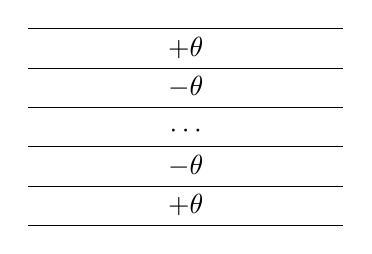
\begin{tikzpicture}
	\draw (0,0) -- (4,0);
	\draw (0,-0.5) -- (4,-0.5) node[midway, above] {$\mathit{+}\theta$};
	\draw (0,-1) -- (4,-1) node[midway, above] {$\mathit{-}\theta$} ;
	\draw (0,-1.5) -- (4,-1.5) node[midway, above] {$\cdots$};
	\draw (0,-2) -- (4,-2) node[midway, above] {$\mathit{-}\theta$};
	\draw (0,-2.5) -- (4,-2.5) node[midway, above] {$\mathit{+}\theta$};
\end{tikzpicture}
\caption{Model for Angle ply laminate}
\end{figure}


\subsection{Maximum stress failure criterion}(MS)


Maximum stress failure theory consists of maximum normal stress theory proposed by Rankine and maximum 
shearing stress theory by Tresca. The stresses applied on a lamina can be resolved into the normal and shear stresses 
in the local axes. If any of the normal or shear stresses in the local axes of a lamina is equal or exceeds the corresponding 
ultimate strengths of the unidirectional lamina, the lamina is considered to be failed. That is,

$\sigma_1 \geq (\sigma _1^{T})_{ult} $ or $\sigma_1 \leq -(\sigma _1^{C})_{ult} $

$\sigma_2 \geq (\sigma _2^{T})_{ult} $ or $\sigma_2 \leq -(\sigma _2^{C})_{ult} $

$\tau_{12} \geq (\tau_{12})_{ult} $  or $\tau_{12} \leq -(\tau_{12})_{ult} $

where $\sigma_1$ and $\sigma_2$ are the normal stresses in the local axes 1 and 2, respectively;
$\tau_{12}$ is the shear stress in the symmetry plane 1-2.

\subsection{Tsai-wu failure criterion}
The TW criterion is one of the most reliable static failure criteria which is derived from the von
Mises yield criterion.  
A lamina is considered to fail
if \begin{equation} \label{eq:tsai_wu}
\begin{split}
	H_1 \sigma_1  & + H_2 \sigma_2 + H_6 \tau_{12} + H_{11}\sigma_1^2 + H_{22} \sigma_2^2 \\
				  & + H_{66}  \tau_{12}^2 + 2H_{12}\sigma_1\sigma_2 < 1
\end{split}
\end{equation}

is violated, where

\begin{equation}
	\begin{split}
		H_{1}&=\frac{1}{\left(\sigma_{1}^{T}\right)_{u l t}}-\frac{1}{\left(\sigma_{1}^{C}\right)_{u l t}} \\
		H_{11}&=\frac{1}{\left(\sigma_{1}^{T}\right)_{u l t}\left(\sigma_{1}^{C}\right)_{u l t}} \\
		H_{2}&=\frac{1}{\left(\sigma_{2}^{T}\right)_{u l t}}-\frac{1}{\left(\sigma_{2}^{C}\right)_{u l t}} \\
		H_{22}&=\frac{1}{\left(\sigma_{2}^{T}\right)_{u l t}\left(\sigma_{2}^{C}\right)_{u l t}} \\
		H_{66}&=\frac{1}{\left(\tau_{12}\right)_{u l t}^{2}} \\
		H_{12}&=-\frac{1}{2} \sqrt{\frac{1}{\left(\sigma_{1}^{T}\right)_{u l
		t}\left(\sigma_{1}^{C}\right)_{u l t}\left(\sigma_{2}^{T}\right)_{u l
		t}\left(\sigma_{2}^{C}\right)_{u l t}}}
	\end{split}
\end{equation}

$H_i$ is the strength tensors of the second order; $H_{ij}$ is the strength
tensors of the fourth order. $\sigma_1$ is the applied normal stress in 
direction 1; $\sigma_2$ is the applied normal stress in the direction 2; and
$\tau_{12}$ is the applied in-plane shear stress.





\begin{figure}
\centering
\begin{tikzpicture}
	\begin{scope}
		%\draw[style=help lines] (-3,-3) grid (3,3);
		\draw (0,0) rectangle (2,3);
		\draw[->] (1.3,1.2) -- (2.6,1.2);
		\draw[->] (1.3,1.2) -- (1.3,3.4);
		\node at (2.2,1) {$X_T$};
		\node at (1.5, 3.2) {$Y_T$};
		\node at (-0.2, 0.9) {$X_C$};
		\node at (1.8, -0.2) {$Y_C$};
	\end{scope}
	\begin{scope}[xshift=6cm,yshift=1.15cm]
		%\draw[style=help lines] (-3,-3) grid (3,3);
		\draw[rotate=30] (0,0) ellipse (2cm and 1cm);
		\draw[->] (0.2,0) -- (0.2,2.2);
		\draw[->] (0.2,0) -- (1.9,0);
		\node at (1.6,-0.2) {$X_T$};
		\node at (0.3, 1.3) {$Y_T$};
		\node at (-1.6, 0) {$X_C$};
		\node at (-0.5, -1.5) {$Y_C$};
	\end{scope}
\end{tikzpicture}
\caption{Schematic failure surfaces for maximum stress and quadratic failure
criteria}
\end{figure}


\subsection{Failure Theories for a Laminate}
If keep increasing the loading applied to a laminate, the laminate will fails. The failure process
of a laminate is more complicate than a lamina, because a laminate consists of multiple plies, and
the fiber orientation, material, thickness of each ply maybe different from the others. In most
situations, some layer fails first and the remains continue to take more loads until all the plies
fail.  If one ply fails, it means this lamina does not contribute to the load carrying capacity of
the laminate. The procedure for finding the first failure ply given follows the fully discounted
method:

\begin{enumerate}
\item Compute the reduced stiffness matrix [Q] referred to as the local axis for each ply using its
	four engineering elastic constants $E_1 $, $E_2 $, $E_{12} $, and $G_{12} $.

\item Calculate the transformed reduced stiffness $[\bar{Q}] $ referring to the global coordinate
	system (x, y) using the reduced stiffness matrix [Q] obtained in step 1 and the ply angle for
	each layer.

\item  Given the thickness and location of each layer, the three laminate stiffness matrices [A],
	[B], and [D] are determined.

\item  Apply the forces and moments, $[N]_{xy}, [M]_{xy} $ solve Equation
	\ref{eq:force_and_moments}, and calculate the middle plane strain $[\sigma ^{0}]_{xy} $ and
	curvature $[k]_{xy} $.

\item Determine the local strain and stress of each layer under the applied load.

\item  Use the ply-by-ply stresses and strains in the Tsai-wu failure theory to find the strength
	ratio, and the layer with smallest strenght ratio is the first failed ply. 
\end{enumerate}

\subsection{Safety factor}
The safety factor, or yield stress, is how much extra load beyond is intended a
composite laminate will actually take. The safey factor is defined as 

\begin{equation} \label{eq:sr}S R=\frac{\text {Maximum Load Which Can Be Applied}}{\text {Load Applied}}
\end{equation}.

\subsection{Safety factor}
The safety factor, or yield stress, is how much extra load beyond is intended a
composite laminate will actually take, which is an indication of the material's
load carrying capacity. If the value is less then 1.0, it means failure. The safey factor is defined as 

\begin{equation} \label{eq:sr}S R=\frac{\text {Maximum Load Which Can Be Applied}}{\text {Load Applied}}
\end{equation}.

The safety factor based on maximum stress theory is calculated by the following
method: first, the principal stresses($\sigma_1^k$,$\sigma_2^k$, and
$\tau_{12}^k$) are obtained by experiment; evaluate the safety factor along each
direction according to equation \ref{eq:sr}; The minimum value among these
safety factors are denoted as the safety factor of the lamina, $SF_{MS}^k$.

\begin{align}
	SF_{MS}^k = \text{min of}
	\begin{cases}
		SF_X^k = 
		\begin{cases}
			\frac{X_t}{\sigma_{11}}, \text{ if } \sigma_{11}>0 \\
			\frac{X_c}{\sigma_{11}}, \text{ if } \sigma_{11}<0 \\
		\end{cases} \\
		SF_Y^k = 
		\begin{cases}
			\frac{Y_t}{\sigma_{22}}, \text{ if } \sigma_{22}>0 \\
			\frac{Y_c}{\sigma_{22}}, \text{ if } \sigma_{22}<0 \\
		\end{cases} \\
		SF_S^k =
		\begin{cases}
			\frac{S}{|\tau_{12}|} \\
		\end{cases} \\
	\end{cases}
\end{align}


Assuming the composite laminate under a in-plane loading f, the corresponding
stress on local stress in direction 1, local stress in direction 2, and shear
stress for the kth lamina are $\sigma_1 SF_{TW}^k$, $\sigma_2SF_{TW}^k$, and $\tau_{12}SF_{TW}^k$,
respectively. Substitute them into the equation \ref{eq:tsai_wu}, the expression
are given by

$a(SF_{TW}^k)^2 + b(SF_{TW}^k) - 1 = 0 $

where 

$a = H_{11}(\sigma_1)^2 + H_{22}(\sigma_2)^2 +H_{66}(\tau_{12})^2 +
2H_{12}\sigma_1 \sigma_2 $

$b = H_1\sigma_1 + H_2 \sigma_2 + H_6 \tau_{12}$

Solve the above equation, the safety factor for the kth lamina is 

$SF_{TW}^k = |\frac{-b+ \sqrt{b^2 + 4a}}{2a}|$.

Then, the minimum of $SF_{TW}^k$ is taken as the safety factor of the
laminate which is written as

$SF_{TW}= \text{ min of } SF_{TW}^k \text{ for } k=1,2,\cdots, m-1,m$ .





In the design of composite material, gradient based optimization techiques are
not appliable in this domain, because the design varaibles, such as fiber
orientation, layer thickness, number of layers etc. are discrete. Genetic
algorithm(GA) can be adopted in the optimization problem becasue it doesn't require
the gradient information. Moreover, the GA has been proved a reliable techique
and widely used in the design of composite material. 

CLT is an classic analytical approach to obtain the stress and stain of
composite material, the disadvantage of this method is quiet cubersome and in
which involves compliate matrix and integration operations. Artificial neural
network(ANN) has been proved a reliable tool in modelling various engineering
system in practice without solving tricky equations and making ideal
assumptions. In this thesis, the ANN is taken to approximate the numberic
results based on CLT and failure theory.

\section{Summary}

In this chapter, we review the classical lamination theory for the stress and
strain analysis in composite material, then related failure theories are
introduced to check whether a composite material would fail or not. In the
following chapters, the CLT would be used to calculate the stress and strain
under in-plane loading, it would also be used to generate the training data for
stress and strain approximation based on neural network; in order to design a
proper composite material, the failure theory are used to decide the feasibility
of composite design.

The rest of this thesis is as follows: in chapter two, we review the classic
lamination theory and related classic lamination theory, which are widely
adopted in the design of composite material; To design composite material, we
provide a new framework of genetic algorithm in chapter three; In chapter four,
this genetic algorith framework is implemented to guide the design of composite
material in two different cases; chapter five discusses about the application of
artificial neural network in composite material for approximating the evaluation
result based on classic lamination theory and failure theory.


